\documentclass[tikz,border=3.14mm]{standalone}
\usetikzlibrary{matrix}
\begin{document}
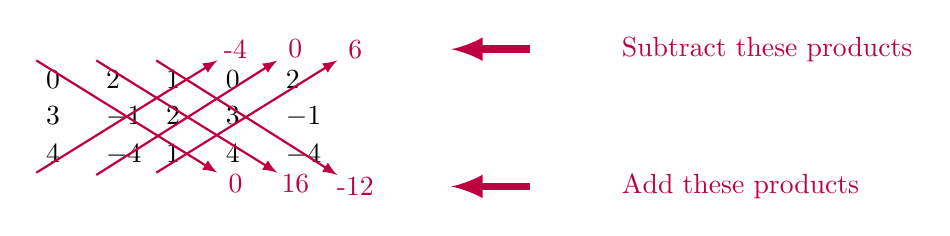
\begin{tikzpicture}
 \edef\lstadd{{0,16,-12}}
 \edef\lstsub{{-4,0,6}}
 \matrix[matrix of math nodes,nodes={text width=1.5em}] (mat)
 {
    0 & 2 & 1 & 0 & 2 \\
    3 & -1 & 2 & 3 & -1\\
    4 & -4 & 1 & 4 & -4\\
 };
 \foreach \X [evaluate=\X as \Y using {int(\X+2)}]in {1,2,3}
 {\pgfmathtruncatemacro{\mylabel}{\lstadd[\X-1]}
 \draw[purple,-latex,thick] (mat-1-\X.north west) -- (mat-3-\Y.south east)
 node[pos=1.1] (LL-\X) {\mylabel};
 \pgfmathtruncatemacro{\mylabel}{\lstsub[\X-1]}
 \draw[purple,-latex,thick] (mat-3-\X.south west) -- (mat-1-\Y.north east)
 node[pos=1.1] (LU-\X) {\mylabel};
 }
 \draw[line width=1mm,purple,latex-,shorten >=1cm,shorten <=1cm]
 (LU-3.east) -- ++ (3,0) node[right] {Subtract these products};
 \draw[line width=1mm,purple,latex-,shorten >=1cm,shorten <=1cm]
 (LL-3.east-|LU-3.east) -- ++ (3,0) node[right] {Add these products};
\end{tikzpicture} 
\end{document}